\documentclass[a4paper,12pt]{article}

\usepackage{mystyle}
\usepackage{gensymb}


\usepackage{scalerel}
\usepackage{stackengine}

\graphicspath{ {images/} }


\definecolor{violet}{RGB}{148, 0, 211}
\definecolor{red}{RGB}{183, 65, 14}
\definecolor{cyan}{RGB}{0, 166, 147}
\definecolor{pink}{RGB}{218, 3, 174}
\definecolor{blue}{RGB}{5, 73, 255}


% https://tex.stackexchange.com/a/101138/135045

\newcommand\widesim[1]{\ThisStyle{%
  \setbox0=\hbox{$\SavedStyle#1$}%
  \stackengine{-.1\LMpt}{$\SavedStyle#1$}{%
    \stretchto{\scaleto{\SavedStyle\mkern.2mu\sim}{.5150\wd0}}{.6\ht0}%
  }{O}{c}{F}{T}{S}%
}}

\newcommand{\BigMiddleTwo}{\;\left|\vphantom{\begin{pmatrix} 0\\0 \end{pmatrix}}\right.\;}
\newcommand{\BigMiddleThree}{\;\left|\vphantom{\begin{pmatrix} 0\\0\\0 \end{pmatrix}}\right.\;}



% https://tex.stackexchange.com/questions/9641/filled-diamondsuit-and-heartsuit
\DeclareSymbolFont{extraup}{U}{zavm}{m}{n}
\DeclareMathSymbol{\varheartsuit}{\mathalpha}{extraup}{86}
\DeclareMathSymbol{\vardiamond}{\mathalpha}{extraup}{87}


% https://tex.stackexchange.com/questions/234942/whats-the-best-way-to-make-a-heart-butt-in-latex
\newcommand{\heart}{\ensuremath\varheartsuit}


% https://tex.stackexchange.com/questions/212710/fill-space-created-by-phantom-with-other-text
\newcommand{\lrhph}[2]{\hphantom{\makebox[#2][l]{}}#1\hphantom{\makebox[#2][l]{}}}



\author{Алексеев Василий}


\title{Семинар 2}
\date{10 + 14 февраля ($\heart$) 2023}


\begin{document}
  \maketitle
  
  \tableofcontents

  \thispagestyle{empty}
  
  \newpage
  
  \pagenumbering{arabic}


  \section{Системы линейных уравнений}

  \subsection{Пример $1$}

  Рассмотрим следующую систему $2 \hm\times 2$:
  \begin{equation}\label{eq:example-1-single-solution}
    \left\{ \begin{aligned}
      &x_1 + x_2 = 0\\
      &x_1 - x_2 = 2
    \end{aligned} \right.
  \end{equation}

  Её также можно переписать в матричном виде:
  \[
    \begin{pmatrix}
      1 & 1\\
      1 & -1
    \end{pmatrix} \begin{pmatrix}
      x_1 \\ x_2
    \end{pmatrix} = \begin{pmatrix}
      0 \\ 2
    \end{pmatrix}
  \]

  Или так:
  \[
    Ax = b
  \]
  где $A \hm= \left(\begin{smallmatrix}1 & 1\\1 & -1\end{smallmatrix}\right)$~---~\emph{матрица системы}, $x \hm= \left(\begin{smallmatrix}x_1 \\ x_2\end{smallmatrix}\right)$~---~столбец из неизвестных, и $b \hm= \left(\begin{smallmatrix}0 \\ 2\end{smallmatrix}\right)$~---~столбец свободных членов.
  В зависимости от того, какой столбец справа, системы делят на два вида: система вида $Ax \hm= b$, $b \hm{\not=} 0$, как в примере, называется \emph{неоднородной}.
  А система вида $Ax \hm= 0$~---~\emph{однородной}.
  В приведённом примере~(\ref{eq:example-1-single-solution}) матрица~$A$ размера $2$ на $2$, то есть в системе два уравнения и две неизвестных.
  В общем же случае матрица системы может быть прямоугольной: $A \hm\in \RR^{m\times n}$, где $m$~---~число уравнений, а $n$~---~число неизвестных.
  И тогда $x \hm\in \RR^n$, $b \hm\in \RR^m$.
  \emph{Решение системы}~---~набор значений переменных, обращающих каждое уравнение системы в верное числовое равенство.
  \emph{Решить систему}~---~значит найти все её решения или показать, что их нет.
  Если хотя бы одно решение есть, система называется \emph{совместной} (иначе~---~несовместной).
  Решение может быть всего одно, или их может быть бесконечно много...\footnote{Может ли у системы $Ax \hm= b$ быть, например, всего два различных решения?}

  Матрица~$A$ системы~(\ref{eq:example-1-single-solution}) квадратная невырожденная.
  По Крамеру, решение такой системы существует и единственно, причём все компоненты решения можно сразу найти по специальной формуле.
  Но решение системы~(\ref{eq:example-1-single-solution}), конечно, можно найти и совсем ``по-простому'', ``как в школе''...
  
  Что можно сделать с системой~(\ref{eq:example-1-single-solution})?
  Можно выразить одну переменную через другую, например, $x_2$ через $x_1$ из первого уравнения.
  Потом подставить во второе, получится уравнение с одной переменной~$x_1$.
  Решить его, а потом найти и зачение второй переменной~$x_2$.
  Это первый из ``школьных приёмов''.
  Ещё был способ ``манипуляций уравнениями''.
  Это когда надо сложить уравнения (возможно, с некоторыми коэффициентами) так, чтобы одна переменная ``пропала''.
  Число переменных таким образом можно ``уменьшить'', чтобы в итоге получилось уравнение лишь с одной неизвестной.

  Решим систему~(\ref{eq:example-1-single-solution}) с помощью ``манипуляций''.
  При этом, по-хорошему, даже после ``уничтожения'' переменной при сложении уравнений мы всё равно должны оставлять систему системой, чтобы можно было найти все неизвестные.
  Будем использовать значок $\sim$ для обозначения перехода от одной системы к другой в результате ``школьной манипуляции'' уравнениями:
  \begin{equation}\label{eq:example-1-solving}
    \left\{
      \begin{aligned}
        &x_1 + x_2 = 0\\
        &x_1 - x_2 = 2
      \end{aligned}
    \right.
    \sim\left\{
      \begin{aligned}
        &x_1 + x_2 = 0\\
        &2x_1 = 2
      \end{aligned}
    \right.
    \sim\left\{
      \begin{aligned}
        &x_1 + x_2 = 0\\
        &x_1 = 1
      \end{aligned}
    \right.
    \sim\left\{
      \begin{aligned}
        &x_2 = -1\\
        &x_1 = 1
      \end{aligned}
    \right.
  \end{equation}
  где сначала прибавили первое уравнение ко второму, потом сократили второе на~$2$, и в конце не подставили найденное значение~$x_2$ в первое уравнение, а снова сложили уравнения, чтобы ``избавиться'' от переменной~---~а именно вычли из первого уже упрощённое второе.

  На самом деле приведённый способ решения это... уже рассмотренный на прошлом семинаре метод Гаусса преобразования строк матрицы!
  Чтобы убедиться в этом, составим \emph{расширенную матрицу} системы, приписав к матрице системы $A$ справа столбец свободных членов $b$.
  Получится матрица вида $(A \hm\mid b)$.
  И проследим, как менялась эта матрица на протяжении решения~(\ref{eq:example-1-solving}).
  То есть на каждом этапе решения выпишем расширенную матрицу для соответствующей упрощённой системы:
  \begin{equation}\label{eq:example-1-matrix-simplification}
    \left(
      \begin{matrix}
        1 & 1\\
        1 & -1
      \end{matrix}
      \BigMiddleTwo
      \begin{matrix}
        0\\
        2
      \end{matrix}
    \right)
    \sim\left(
      \begin{matrix}
        1 & 1\\
        2 & 0
      \end{matrix}
      \BigMiddleTwo
      \begin{matrix}
        0\\
        2
      \end{matrix}
    \right)
    \sim\left(
      \begin{matrix}
        1 & 1\\
        1 & 0
      \end{matrix}
      \BigMiddleTwo
      \begin{matrix}
        0\\
        1
      \end{matrix}
    \right)
    \sim\left(
      \begin{matrix}
        0 & 1\\
        1 & 0
      \end{matrix}
      \BigMiddleTwo
      \begin{matrix}
        -1\\
        1
      \end{matrix}
    \right)
  \end{equation}

  Видно, что школьный приём ``манипуляций'' уравнениями~---~это по сути элементарные преобразования строк расширенной матрицы системы с целью упрощения, ``чистки столбцов''.
  То есть можно думать, что решение системы словно разворачивается параллельно ``в двух плоскостях'': с одной стороны, упрощение уравнений системы, ``уничтожение'' переменных; с другой~---~преобразование строк расширенной матрицы при приведении матрицы системы к упрощённому виду.
  В процессе решения каждой системе уравнений после преобразования соответствует расширенная матрица.
  И наоборот: каждой расширенной матрице, получающейся в результате упрощения исходной методом Гаусса, соответствует система уравнений.

  По-хорошему, преобразования строк матрицы~(\ref{eq:example-1-matrix-simplification}) ещё не доведены до конца~---~до получения упрощённого вида матрицы системы (матрица $A$ была невырожденная, поэтому её упрощённый вид есть просто единичная матрица того же порядка) остаётся поменять местами строки:
  \[
    \left(
      \begin{matrix}
        1 & 0\\
        0 & 1
      \end{matrix}
      \BigMiddleTwo
      \begin{matrix}
        1\\
        -1
      \end{matrix}
    \right)
  \]

  И соответствующая система уравнений (где просто переменные идут ``по порядку''):
  \[
    \left\{
      \begin{aligned}
        &x_1 = 1\\
        &x_2 = -1
      \end{aligned}
    \right.
  \]

  Таким образом, основное, что будет дальше в конспекте~---~это снова решение систем линейных уравнений, но на этот методом Гаусса (снова элементарные пребразования строк).
  Новое~---~как другой взгляд на старое.
  Под другим углом, с другой стороны, в других обозначениях...

  % Перед тем, как продолжить, отметим ещё два понятия.
  % Система $Ax \hm= 0$ называется \emph{однородной}

  
  \subsection{Пример $8$}  % $\infty$

  Рассмотрим другую систему (``модифицированная'' первая система~(\ref{eq:example-1-single-solution})):
  \begin{equation}\label{eq:example-2-infty-solutions}
    \left\{ \begin{aligned}
      &x_1 + x_2 + x_3 \hphantom{{} + x_4} = 0\\
      &x_1 - x_2 + \hphantom{x_3 + {}} x_4 = 2\\
      &\hphantom{x_1 + } 2x_2 + x_3 - x_4 = -2
    \end{aligned} \right.
  \end{equation}

  В системе три уравнения, четыре неизвестных.
  Она решается?
  % Система~(\ref{eq:example-2-infty-solutions}) похожа на~(\ref{eq:example-1-single-solution}): возьмём $x_3 \hm= x_4 hm= 0$, тогда подходящая пара $(x_1, x_2)$ точно существует и единственна.
  % Возьмём другие $x_3$ и $x_4$ и перенесём их направо в первом и втором уравнениях системы~(\ref{eq:example-2-infty-solutions})~---~снова получим систему с единственным решением для $x_1$ и $x_2$.
  % Таким образом, решение у системы~(\ref{eq:example-2-infty-solutions}), причём их бесконечно много: беря произвольные $x_3$ и $x_4$, получаем по ним $x_1$ и $x_2$, и вместе в совокупности эти четыре значения дают возможное решение.
  % Как описать это бесконечное множество решений?
  Чтобы выяснить это (и найти решение, если оно есть), применим тот же метод Гаусса.
  Матрица системы $A \hm\in \RR^{3\times 4}$ в данном случае прямоугольная\footnote{Считаем, что ``подвоха'' по умолчанию нет, то есть что кроме переменных, представленных в системе с ненулевыми коэффициентами ($x_1$, $x_2$, $x_3$, $x_4$), больше неизвестных нет.}.
  Поэтому единичную матрицу из $A$ с помощью элементарных преобразований строк не получить.
  Но матрицу~$A$ можно упростить, получив в некоторых $r$ её столбцах единичную матрицу и оставив нулевыми все строки с номерами больше $r$ (\emph{упрощённый вид} матрицы, число $r$ при этом будет равно рангу $A$).

  % https://tex.stackexchange.com/questions/212710/fill-space-created-by-phantom-with-other-text
  % TODO: "handcrafted spaces" around MiddleThree
  \begin{equation*}
  \begin{split}
    \left(
      \begin{matrix}
        1 & 1 & 1 & 0\\
        1 & -1 & 0 & 1\\
        0 & 2 & 1 & -1
      \end{matrix}
      \BigMiddleThree
      \begin{matrix}
        0\\
        2\\
        -2
      \end{matrix}
    \right)
    %%
    \xrightarrow{(2) = (2) - (1)} &\left(
      \begin{matrix}
        1 & 1 & 1 & 0\\
        0 & -2 & -1 & 1\\
        0 & 2 & \lrhph{1}{5.25pt} & -1
      \end{matrix}
      \BigMiddleThree
      \begin{matrix}
        0\\
        2\\
        -2
      \end{matrix}
    \right)\\
    %%
    \xrightarrow{(3) = (3) + (2)} &\left(
      \begin{matrix}
        1 & 1 & 1 & 0\\
        0 & -2 & -1 & 1\\
        \textcolor{blue}{0} & \textcolor{blue}{0} & \textcolor{blue}{0} & \lrhph{\textcolor{blue}{0}}{5.25pt}
      \end{matrix}
      \BigMiddleThree
      \begin{matrix}
        0\\
        2\\
        \lrhph{\textcolor{pink}{0}}{4pt}
      \end{matrix}
    \right)\\
    %%
    \xrightarrow{(2) = -1/2 \cdot (2)} &\left(
      \begin{matrix}
        1 & 1 & 1 & 0\\
        0 & 1 & 1/2 & -1/2\\
        0 & 0 & 0 & 0
      \end{matrix}
      \BigMiddleThree
      \begin{matrix}
        0\\
        -1\\
        0
      \end{matrix}
    \right)
    %%
    \xrightarrow{(1) = (1) - (2)} \left(
      \begin{matrix}
        \bds 1 & \bds 0 & 1/2 & 1/2\\
        \bds 0 & \bds 1 & 1/2 & -1/2\\
        0 & 0 & 0 & 0
      \end{matrix}
      \BigMiddleThree
      \begin{matrix}
        1\\
        -1\\
        0
      \end{matrix}
    \right)
  \end{split}
  \end{equation*}

  Пришли к упрощённой матрице\footnote{При этом последнюю строчку, нулевую, да, можно как бы вообще ``выкинуть''... В этом примере.}~$A'$ и преобразованному аналогичным образом столбцу~$b'$:
  \[
    A' = \begin{pmatrix}
      1 & 0 & 1/2 & 1/2\\
      0 & 1 & 1/2 & -1/2\\
      0 & 0 & 0 & 0
    \end{pmatrix},\quad b' = \begin{pmatrix}
      1\\
      -1\\
      0
    \end{pmatrix}
  \]
  
  Выпишем систему, соответствующую расширенной матрице~$(A' \hm\mid b')$:
  \[
    \left\{
      \begin{aligned}
        &x_1 + 1/2 x_3 + 1/2 x_4 = 1\\
        &x_2 + 1/2 x_3 - 1/2 x_4 = -1
      \end{aligned}
    \right.
  \]

  Переменные, которым соответствуют столбцы единичной матрицы в упрощённом виде матрицы~$A'$, называются \emph{базисными}.
  (Базисная подматрица, базисные столбцы~---~базисные переменные.)
  В нашем случае это $x_1$ и $x_2$.
  Остальные переменные ($x_3$ и $x_4$) называются \emph{свободными}, или параметрическими.
  Почему такое название, будет понятно далее.

  Видно, что базисные переменные легко выражаются через оставшиеся:
  \[
    \left\{
      \begin{aligned}
        &x_1 = 1 - 1/2 x_3 - 1/2 x_4\\
        &x_2 = -1 - 1/2 x_3 + 1/2 x_4
      \end{aligned}
    \right.
  \]

  На самом деле решение уже получено.
  Например, берём $x_3 \hm= 0$, $x_4 \hm= 0$, получаем по приведённым формулам значения $x_1$ и $x_2$, все вместе они дают одно из решений.
  Берём другие, \emph{произвольные}, значения $x_3$ и $x_4$, снова получаем по формулам $x_1$ и $x_2$, находим ещё одно решение.

  Описать всё бесконечное множество решений можно следующим образом (введя параметры, пробегающие всё $\RR$, в качестве значений свободных неизвестных):
  \[
    \left\{
      \begin{aligned}
        &x_3 = 2 t_1 \in \RR\\
        &x_4 = 2 t_2 \in \RR\\
        &x_1 = 1 - t_1 - t_2\\
        &x_2 = -1 - t_1 + t_2
      \end{aligned}
    \right.
  \]

  Запишем решение в виде столбца:
  \begin{equation*}
  \begin{split}
    \begin{pmatrix}
      x_1\\
      x_2\\
      x_3\\
      x_4
    \end{pmatrix}
    = &\begin{pmatrix}
      1 - t_1 - t_2\\
      -1 - t_1 + t_2\\
      2t_1\\
      2t_2
    \end{pmatrix}\\
    = &\underbrace{
        \begin{pmatrix}
          1 \\ -1 \\ 0 \\ 0
        \end{pmatrix}
      }_{\substack{\tiny \mbox{Частное решение неоднородной системы}\\ \tiny \mbox{(решение при нулевых свободных переменных)}}}
    + \underbrace{
        \begin{pmatrix}
          -1 \\ -1 \\ 2 \\ 0
        \end{pmatrix} t_1 + \begin{pmatrix}
          -1 \\ 1 \\ 0 \\ 2
        \end{pmatrix} t_2
      }_{\substack{\tiny \mbox{Общее решение однородной системы}\\ \tiny \mbox{(решение при нулевом столбце свободных членов)}}}\\
    = &\begin{pmatrix}
      1 \\ -1 \\ 0 \\ 0
    \end{pmatrix}
    + \underbrace{
        \begin{pmatrix}
          -1 & -1\\
          -1 & 1\\
          2 & 0\\
          0 & 2
        \end{pmatrix}
      }_{\substack{\tiny \mbox{Фундаментальная матрица}\\ \tiny \mbox{(её столбцы~---~базис в пространстве} \\ \tiny \mbox{решений однородной системы)}}} \begin{pmatrix} t_1 \\ t_2 \end{pmatrix}
  \end{split}
  \end{equation*}

  Столбцы, состоящие из коэффициентов перед параметрами~$t_1$ и $t_2$, можно собрать в матрицу, которая называется \emph{фундаментальной матрицей, соответствующей однородной системе $Ax \hm= 0$}.
  Можно заметить, что эти столбцы~---~\emph{решения однородной системы}; ещё видно, что они \emph{линейно независимые}; и \emph{любое решение однородной представимо как их линейная комбинация}.
  
  Базисных переменных всего $r$~---~количество, равное рангу~$A$.
  Значит, свободных переменных будет $n \hm- r$.
  Но количество свободных как раз и определяет число столбцов фундаментальной матрицы~$\Phi$.
  Таким образом, размер фундаментальной должен быть $n \hm\times (n \hm- r)$.
  ``Наполнение'' же фундаментальной матрицы для данной системы $Ax \hm= 0$ \emph{неоднозначно}: главное, чтобы выполнялись условия на столбцы.

  Итак, решений у системы~(\ref{eq:example-2-infty-solutions}) оказалось бесконечно много.
  (При этом ``бесконечно много'' $\hm{\not=}$ ``произвольные''.)
  Однако не всегда всё складывается так хорошо...


  \subsection{Пример $0$}

  Рассмотрим ещё одну систему (``модификация'' второй~(\ref{eq:example-2-infty-solutions})):
  \begin{equation}\label{eq:example-3-no-solutions}
    \left\{ \begin{aligned}
      &x_1 + x_2 + x_3 \hphantom{{} + x_4} = 0\\
      &x_1 - x_2 + \hphantom{x_3 + {}} x_4 = 2\\
      &\hphantom{x_1 + } 2x_2 + x_3 - x_4 = \bds{-1}
    \end{aligned} \right.
  \end{equation}

  Есть ли у неё решения?
  Снова попытаемся упростить методом Гаусса:
  % TODO: handcrafted spaces around MiddleTreee
  \begin{equation*}
  \begin{split}
    &\left(
      \begin{matrix}
        1 & 1 & \lrhph{1}{4pt} & \lrhph{0}{7pt}\\
        1 & -1 & 0 & 1\\
        0 & 2 & 1 & -1
      \end{matrix}
      \BigMiddleThree
      \begin{matrix}
        0\\
        2\\
        -1
      \end{matrix}
    \right)\\
    %%
    \xrightarrow{(2) = (2) - (1)} &\left(
      \begin{matrix}
        1 & 1 & 1 & 0\\
        0 & -2 & -1 & 1\\
        0 & 2 & \lrhph{1}{7pt} & {-1}
      \end{matrix}
      \BigMiddleThree
      \begin{matrix}
        0\\
        2\\
        -1
      \end{matrix}
    \right)\\
    %%
    \xrightarrow{(3) = (3) + (2)} &\left(
      \begin{matrix}
        1 & 1 & 1 & 0\\
        0 & -2 & -1 & 1\\
        \textcolor{blue}{0} & \textcolor{blue}{0} & \textcolor{blue}{0} & \lrhph{\textcolor{blue}{0}}{7pt}
      \end{matrix}
      \BigMiddleThree
      \begin{matrix}
        0\\
        2\\
        \lrhph{\textcolor{pink}{1}}{4pt}
      \end{matrix}
    \right)
  \end{split}
  \end{equation*}

  На этом можно закончить.
  Потому что давайте посмотрим на получившуюся систему уравнений:
  \[
    \left\{
      \begin{aligned}
        &x_1 + x_2 + x_3 = 0\\
        &-2x_2 - x_3 + x_4 = 2\\
        &\boxed{0 = 1} \mbox{\ ---~``конец''}
      \end{aligned}
    \right.
  \]

  Получили противоречие: слева в преобразованной матрице системы~$A'$ строчка нулевая, а соответствующая компонента преобразованного столбца~$b'$ нулю не равна.
  Раньше такого в процессе преобразований расширенной матрицы~$(A \hm\mid b)$ не было~---~система решалась.
  Противоречие появилось~---~решений нет.

  Есть несколько вариантов сформулировать это наблюдение ``по-умному''.

  \begin{theorem}[Кронекера~--~Капелли]
    Система $Ax \hm= b$ совместна $\Leftrightarrow \Rg(A) \hm= \Rg(A \hm\mid b)$.
  \end{theorem}

  Ранг матрицы~$A$~---~максимальное количество линейно независимых столбцов (базисные столбцы).
  Если приписывание нового столбца не меняет ранг, это значит, что новый столбец раскладывается по базисным.
  Но если в упрощённом виде у всех базисных какая-то компонента нулевая (нулевая строка в матрице~$A'$), а в приписанном столбце после тех же преобразований стоит не ноль, то этот столбец~$b'$, очевидно, никак не может быть разложен по базисным~$A'$ (а значит, и исходный~$b$ не мог быть разложен по базисным исходной~$A$), то есть максимальное число линейно независимых столбцов увеличивается, и ранг другой.

  \begin{theorem}[Фредгольма]
    Система $Ax \hm= b$ совместна $\Leftrightarrow (y^T A \hm=0_{1\times n} \hm\rightarrow y^T b \hm= 0_{1\times 1})$.
  \end{theorem}

  Иными словами, что это значит, если в матрице~$A$ удалось занулить какую-то строчку?
  Это значит, что она может быть разложена в линейную комбинацию других.
  То есть строчки~$A$ можно сложить с некоторыми коэффициентами так, чтобы получить нулевую.
  Это сложение строк с коэффициентами можно представить как умножение матрицы~$A$ слева на строку\footnote{Считается как бы, что маленькие строчные буквы: $x$, $y$, ...~---~по умолчанию представляют столбцы (``координатный \emph{столбец} вектора в базисе''~---~раньше у вектор-столбца тоже была ``особая роль''). Тогда $y^T$ будет строчкой.} из коэффициентов $y^T \hm\in \RR^{1\times m}$.
  Если в результате такого действия в расширенной матрице справа окажется не ноль, то есть $y^T b \hm{\not=} 0$, то получим противоречие.

  \begin{example}
    Если $y^T A \hm= 0$ только при нулевой строчке $y^T$, то это значит, что строки матрицы~$A$ линейно независимы.
    Очевидно, что в этом случае обязательно и $y^T b \hm= 0$, и решение у системы $Ax \hm= b$ есть.

    В системе~(\ref{eq:example-3-no-solutions}), ``можно заметить'', третья строчка есть первая минус вторая.
    То есть, например, при $y^T \hm= (1, -1, -1)$ имеем $y^T A \hm= 0$.
    Однако $y^T b \hm= -1 \hm{\not=} 0$.
  \end{example}
  
  
  \section{Задачи}
  
  \subsection{\# 17.1(4)}
  
  Выписать расширенную матрицу.
  Решить систему уравнений:
  \[
    \left\{
    \begin{aligned}
      &y + 3z = -1\\
      &2x + 3y + 5z = 3\\
      &3x + 5y + 7z = 6
    \end{aligned}
    \right.
  \]

  % TODO: crazy handcrafted spacing - looks good in PDF, but bad (very bad) in TeX...
  \begin{solution}
    \begin{equation*}
    \begin{split}
      &\left(
          \begin{matrix}
            0 & \textcolor{pink}{\bds 1} & 3\\
            2 & \textcolor{blue}{\bds 3} & 5\\
            3 & \textcolor{blue}{\bds 5} & \lrhph{7}{6pt}
          \end{matrix}
          \BigMiddleThree
          \begin{matrix}
            -1\\
            3\\
            6
          \end{matrix}
        \right)
      \xrightarrow{\substack{(2) = (2) - 3 \cdot (1)\\(3) = (3) - 5 \cdot (1)}} \left(
          \begin{matrix}
            0 & 1 & \lrhph{3}{5pt}\\
            2 & 0 & -4\\
            3 & 0 & -8
          \end{matrix}
          \BigMiddleThree
          \begin{matrix}
            -1\\
            6\\
            11
          \end{matrix}
        \right)\\
      \xrightarrow{(2) = (2) / 2} &\left(
          \begin{matrix}
            0 & 1 & \lrhph{3}{6pt}\\
            \textcolor{pink}{\bds 1} & 0 & -2\\
            \textcolor{blue}{\bds 3} & 0 & -8
          \end{matrix}
          \BigMiddleThree
          \begin{matrix}
            -1\\
            3\\
            11
          \end{matrix}
        \right)
      \xrightarrow{(3) = (3) - 3 \cdot (2)} \left(
          \begin{matrix}
            0 & 1 & \lrhph{3}{5pt}\\
            1 & 0 & -2\\
            0 & 0 & -2
          \end{matrix}
          \BigMiddleThree
          \begin{matrix}
            -1\\
            3\\
            2
          \end{matrix}
        \right)\\
      \xrightarrow{(3) = -1/2 \cdot (3)} &\left(
          \begin{matrix}
            0 & 1 & \lrhph{\textcolor{blue}{\bds 3}}{6pt}\\
            1 & 0 & \textcolor{blue}{\bds{-2}}\\
            0 & 0 & \textcolor{pink}{\bds 1}
          \end{matrix}
          \BigMiddleThree
          \begin{matrix}
            -1\\
            3\\
            -1
          \end{matrix}
        \right)
      \xrightarrow{\substack{(1) = (1) - 3 \cdot (3)\\(2) = (2) + 2 \cdot (3)}} \left(
          \begin{matrix}
            0 & 1 & 0\\
            1 & 0 & 0\\
            0 & 0 & \lrhph{1}{5pt}
          \end{matrix}
          \BigMiddleThree
          \begin{matrix}
            2\\
            1\\
            -1
          \end{matrix}
        \right)\\
    \end{split}
    \end{equation*}
    
    Упрощённой матрице соответствует система
    \[
      \left\{
        \begin{aligned}
          &y = 2\\
          &x = 1\\
          &z = -1\\
        \end{aligned}
      \right.
    \]
    то есть решение есть $(1, 2, -1)^T$.
  \end{solution}


  \subsection{\# 19.19(1)}
  
  Расширенная матрица системы содержит параметр:
  \[
    (A \mid b) = \left(
      \begin{matrix}
        1 & 2 & 3\\
        2 & 3 & 4\\
        3 & 4 & 5
      \end{matrix}
      \BigMiddleThree
      \begin{matrix}
        \alpha\\
        \alpha^2\\
        \alpha^3
      \end{matrix}
    \right)
  \]

  Найти все значения параметра~$\alpha$, при которых система $Ax \hm= b$ совместна, и решить.
  
  \begin{solution}
    ``Заметим'', что третья строчка есть разность удвоенной второй и первой.
    Таким образом, преобразования матрицы можно начать ``нестандартно'':
    \[
      \left(
        \begin{matrix}
          1 & 2 & 3\\
          2 & 3 & 4\\
          3 & 4 & 5
        \end{matrix}
        \BigMiddleThree
        \begin{matrix}
          \alpha\\
          \alpha^2\\
          \alpha^3
        \end{matrix}
      \right)
      \sim \left(
        \begin{matrix}
          1 & 2 & 3\\
          2 & 3 & 4\\
          0 & 0 & 0
        \end{matrix}
        \BigMiddleThree
        \begin{matrix}
          \alpha\\
          \alpha^2\\
          \alpha^3 - 2\alpha^2 + \alpha
        \end{matrix}
      \right)
    \]

    Очевидно, первые две строки преобразованной матрицы~$A'$ линейно независимы (нулевой строки там уже не получится).
    То есть $\Rg A \hm= 2$.
    Поэтому по теореме Кронекера~--~Капелли (или по теореме Фредгольма, или просто потому, что не может в ``нормальной'' системе получиться $0 \hm= 1$):
    \[
      \alpha^3 - 2\alpha^2 + \alpha = 0
      \Leftrightarrow \left[
        \begin{aligned}
          &\alpha = 0\\
          &\alpha = 1
        \end{aligned}
      \right.
    \]

    При $\alpha \hm= 0$ получаем однородную систему (выпишем сразу матрицу с занулённой третьей строчкой):
    \begin{equation}\label{19-19-sys-homo}
      \left(
        \begin{matrix}
          1 & 2 & 3\\
          2 & 3 & 4\\
          0 & 0 & 0
        \end{matrix}
        \BigMiddleThree
        \begin{matrix}
          0\\
          0\\
          0
        \end{matrix}
      \right)
    \end{equation}
    
    При $\alpha \hm= 1$~---~неоднородную:
    \begin{equation}\label{19-19-sys-hetero}
      \left(
        \begin{matrix}
          1 & 2 & 3\\
          2 & 3 & 4\\
          0 & 0 & 0
        \end{matrix}
        \BigMiddleThree
        \begin{matrix}
          1\\
          1\\
          0
        \end{matrix}
      \right)
    \end{equation}

    Решим сначала, например, однородную~(\ref{19-19-sys-homo}):
    \[
      \left(
        \begin{matrix}
          1 & 2 & 3\\
          2 & 3 & 4\\
          0 & 0 & 0
        \end{matrix}
        \BigMiddleThree
        \begin{matrix}
          0\\
          0\\
          0
        \end{matrix}
      \right)
      \sim \left(
        \begin{matrix}
          1 & 2 & 3\\
          0 & -1 & -2\\
          0 & 0 & 0
        \end{matrix}
        \BigMiddleThree
        \begin{matrix}
          0\\
          0\\
          0
        \end{matrix}
      \right)
      \sim \left(
        \begin{matrix}
          1 & 0 & -1\\
          0 & 1 & 2\\
          0 & 0 & 0
        \end{matrix}
        \BigMiddleThree
        \begin{matrix}
          0\\
          0\\
          0
        \end{matrix}
      \right)
    \]
    
    Преобразованная система:
    \[
      \left\{
        \begin{aligned}
          &x_1 - x_3 = 0\\
          &x_2 + 2x_3 = 0
        \end{aligned}
      \right.
      \leftrightarrow
      \left\{
        \begin{aligned}
          &x_1 = x_3\\
          &x_2 = -2x_3
        \end{aligned}
      \right.
    \]

    Поэтому решение:
    \[
      \begin{pmatrix}
        x_1\\
        x_2\\
        x_3
      \end{pmatrix} = \begin{pmatrix}
        1\\
        -2\\
        1
      \end{pmatrix} t
    \]

    Если же внимательно посмотреть на неоднородную~(\ref{19-19-sys-hetero}), то можно увидеть частное решение $(-1, 1, 0)^T$.
    Значит, имея общее решение однородной и частное неоднородной, можно сразу выписать общее решение неоднородной\footnote{А можно было бы, наоборот, ``по-честному'' решить сначала неоднородную, и потом сразу выписать решение однородной. В любом случае, в этом номере не обязательно решать от начала и до конца, по Гауссу, две системы при разных $\alpha$.}:
    \[
      \begin{pmatrix}
        x_1\\
        x_2\\
        x_3
      \end{pmatrix} = \begin{pmatrix}
        -1\\
        1\\
        0
      \end{pmatrix} + \begin{pmatrix}
        1\\
        -2\\
        1
      \end{pmatrix} t
    \]
  \end{solution}

  
  % TODO: task on on page, solution starts on the other page
  \newpage
  
  \subsection{\# 18.17(1)}
  
  Найти однородную систему, для которой фундаментальной является матрица $\Phi$ следующего вида:
  \[
    \Phi = \begin{pmatrix}
      3 & 1\\
      2 & 1\\
      1 & 0
    \end{pmatrix}
  \]
  
  \begin{solution}
    \hphantom{X}\par  % TODO: new line after "`Solution"'
    
    \paragraph{Способ 1: Решение системы ``наоборот''.}
    
    Размер фундаментальной матрицы $3 \hm\times 2$.
    Значит, неизвестных в системе всего $3$.
    А ранг самой матрицы $A$ равен $3 \hm- 2 \hm= 1$.
    То есть в матрице всего ``одна строчка'' (может быть и больше~---~главное, чтоб ранг был равен одному, то есть чтоб ``информативная'' была всего одна строчка).
    
    При данной фундаментальной матрице $\Phi$ общее решение однородной системы выражается как линейная комбинация её столбцов:
    \begin{equation*}
    \begin{split}
      \begin{pmatrix} x_1 \\ x_2 \\ x_1 \end{pmatrix}
      = x = \Phi h = \begin{pmatrix}
          3 & 1\\
          2 & 1\\
          1 & 0
        \end{pmatrix} \begin{pmatrix}
          h_1 \\ h_2
        \end{pmatrix}
      = h_1 \cdot \begin{pmatrix} 3 \\ 2 \\ 1 \end{pmatrix} +
         h_2 \cdot \begin{pmatrix} 1 \\ 1 \\ 0 \end{pmatrix} \quad h_1, h_2 \in \RR
    \end{split}
    \end{equation*}
    
    Это значит, что при определённом наборе чисел $(x_1, x_2, x_3)$ коэффициенты разложения $h_1$ и $h_2$ по столбцам фундаментальной матрицы $\Phi$ найдутся тогда и только тогда, когда вектор $(x_1, x_2, x_3)$ будет решением системы $A x \hm= 0$.
    
    Перепишем выражение для общего решения выше в виде системы:
    \[
      \left\{
        \begin{aligned}
          &x_1 = 3h_1 + h_2\\
          &x_2 = 2h_1 + h_2\\
          &x_3 = h_1
        \end{aligned}
      \right.
    \]
    
    Таким образом, можно попытаться решить эту систему относительно $h_1$ и $h_2$.
    И в процессе решения получить условие на компоненты $x_1, x_2, x_3$, при которых система будет разрешима.
    Можно воспользоваться методом Гаусса.
    Либо просто ``поиграть с уравнениями'' (что в целом одно и то же):
    \[
      \left\{
        \begin{aligned}
          &x_1 = 3h_1 + h_2\\
          &x_2 = 2h_1 + h_2\\
          &x_3 = h_1
        \end{aligned}
      \right. \Leftrightarrow \left\{
        \begin{aligned}
          &x_1 - x_2 = h_1\\
          &x_2 = 2h_1 + h_2\\
          &x_3 = h_1
        \end{aligned}
      \right. \Leftrightarrow \left\{
        \begin{aligned}
          &x_1 - x_2 = x_3\\
          &h_2 = x_2 - 2h_1 = x_2 - 2x_3\\
          &h_1 = x_3
        \end{aligned}
      \right.
    \]
    
    Условие разрешимости (ограничение на компоненты вектора $x$, чтобы его можно было найти коэффициенты разложения $h_1$ и $h_2$): $\boxed{x_1 - x_2 = x_3}$.
    Если указанное соотношение между $(x_1, x_2, x_3) \hm= x$ не выполняется, коэффициенты $h_1$ и $h_2$ найти нельзя ($x$~---~не решение $Ax \hm= 0$).
    Иначе~---~коэффициенты $h_1$ и $h_2$ найти можно и потому $x \hm= (x_1, x_2, x_3)$~---~решение $Ax \hm= 0$.
    В итоге матрицу $A$ можно взять в виде:
    \[
      A = (1, -1, -1)
    \]

    Очевидно, ответ не однозначен: строчку можно несколько раз продублировать, даже с некоторым ненулевым коэффициентом (см. задачу~(\ref{sec:18-18}) далее).
    
    \bigskip
    
    \paragraph{Способ 2: ``Обычное'' решение системы...}
    
    В условии дана фундаментальная матрица.
    То есть её столбцы~---~решения однородной системы.
    Это значит, что в уравнение $Ax \hm= 0$ можно подставить вместо $x$ поочерёдно столбцы $\Phi$, и это будет давать верные числовые равенства.
    Пусть в матрице $A$ всего $m$ строк (и $3$ столбца).
    Тогда $Ax \hm= 0$ в виде системы можно записать так:
    \[
      \left\{
        \begin{aligned}
          &a_{11} x_1 + a_{12} x_2 + a_{13} x_3 = 0\\
          &a_{21} x_1 + a_{22} x_2 + a_{23} x_3 = 0\\
          &\ldots\\
          &a_{m1} x_1 + a_{m2} x_2 + a_{m3} x_3 = 0
        \end{aligned}
      \right.
    \]
    
    Подставляем сюда вместо $x_1$, $x_2$ и $x_3$ компоненты первого столбца $\Phi$:
    \[
      \left\{
        \begin{aligned}
          &3 a_{11} + 2 a_{12} + a_{13} = 0\\
          &3 a_{21} + 2 a_{22} + a_{23} = 0\\
          &\ldots
        \end{aligned}
      \right.
    \]
    
    И компоненты второго столбца $\Phi$:
    \[
      \left\{
        \begin{aligned}
          &a_{11} + a_{12} \hphantom{+ a_{13}} = 0\\
          &a_{21} + a_{22} \hphantom{+ a_{23}} = 0\\
          &\ldots
        \end{aligned}
      \right.
    \]
    
    Отсюда надо найти коэффициенты $a_{ij}$, составляющие матрицу $A$.
    Чтобы это сделать, можно сгруппировать уравнения из двух систем по строчкам:
    \[
      \left\{
        \begin{aligned}
          &\left\{
            \begin{aligned}
              &3 a_{11} + 2 a_{12} + a_{13} = 0\\
              &\hphantom{3}a_{11} + \hphantom{2}a_{12} \hphantom{+ a_{13}} = 0
            \end{aligned}
          \right.\\
          &\ldots
        \end{aligned}
      \right.
    \]
    
    В каждой такой паре уравнений можно принять первую и вторую переменные за базисные (выразить через третью).
    В итоге строки матрицы $A$ должны выглядеть так:
    \[
      A = \begin{pmatrix}
        -a_{13} & a_{13} & a_{13}\\
        -a_{23} & a_{23} & a_{23}\\
        \ldots
      \end{pmatrix}
    \]
    
    Три столбца линейно зависимы: например, первый и второй очевидным образом выражаются через третий.
    Поэтому максимальное число линейно независимых строк в матрице $A$~---~одна строчка (строчный ранг совпадает со столбцовым).
    Поэтому остаётся составить подходящую строку коэффициентов.
    Например,
    \[
      A = \begin{pmatrix}
        -1 & 1 & 1
      \end{pmatrix}
    \]
    
    И тогда ``система'' уравнений:
    \[
      \left\{
        \begin{aligned}
          &-x_1 + x_2 + x_3 = 0
        \end{aligned}
      \right.
    \]
  \end{solution}
  
  
  \section{Дополнение}
  \subsection{\# 18.18}
  \label{sec:18-18}
  
  Найти \emph{все} однородные системы уравнений, эквивалентные данной системе $Ax \hm= 0$.
  
  \begin{solution}
    Надо найти совокупность матриц $B$, таких что $Bx \hm= 0 \hm\Leftrightarrow Ax \hm= 0$.
    Очевидно, столбцов в матрице $B$ столько же, сколько и в данной в условии $A$ (число неизвестных).
    Пусть размер матрицы $A$ есть $m$ строк на $n$ столбцов.
    А размер матрицы $B$ пусть $l$ строк на $n$ столбцов.
    Сколько строк $l$ должно быть в матрице $B$, дающей такое же множество решений, что и $A$?
    
    ``Информативные'' строки матрицы $A$ должны сохраниться (их количество~---~ранг матрицы $r$).
    И к ним можно добавить сколько угодно ``лишних'' (или убрать из исходной системы, если строки $A$ линейно зависимы).
    Таким образом, $l \hm\geq r$.
    При этом $r$ ``информативных'' строк $B$~---~это преобразованные $r$ базисных (каких-то) строк матрицы $A$.
    Остальные строки $B$ (если есть)~---~это произвольные линейные комбинации базисных строк $A$ (\ref{fig:colourful-rows}).

    \begin{figure}[h]
      \centering
    
      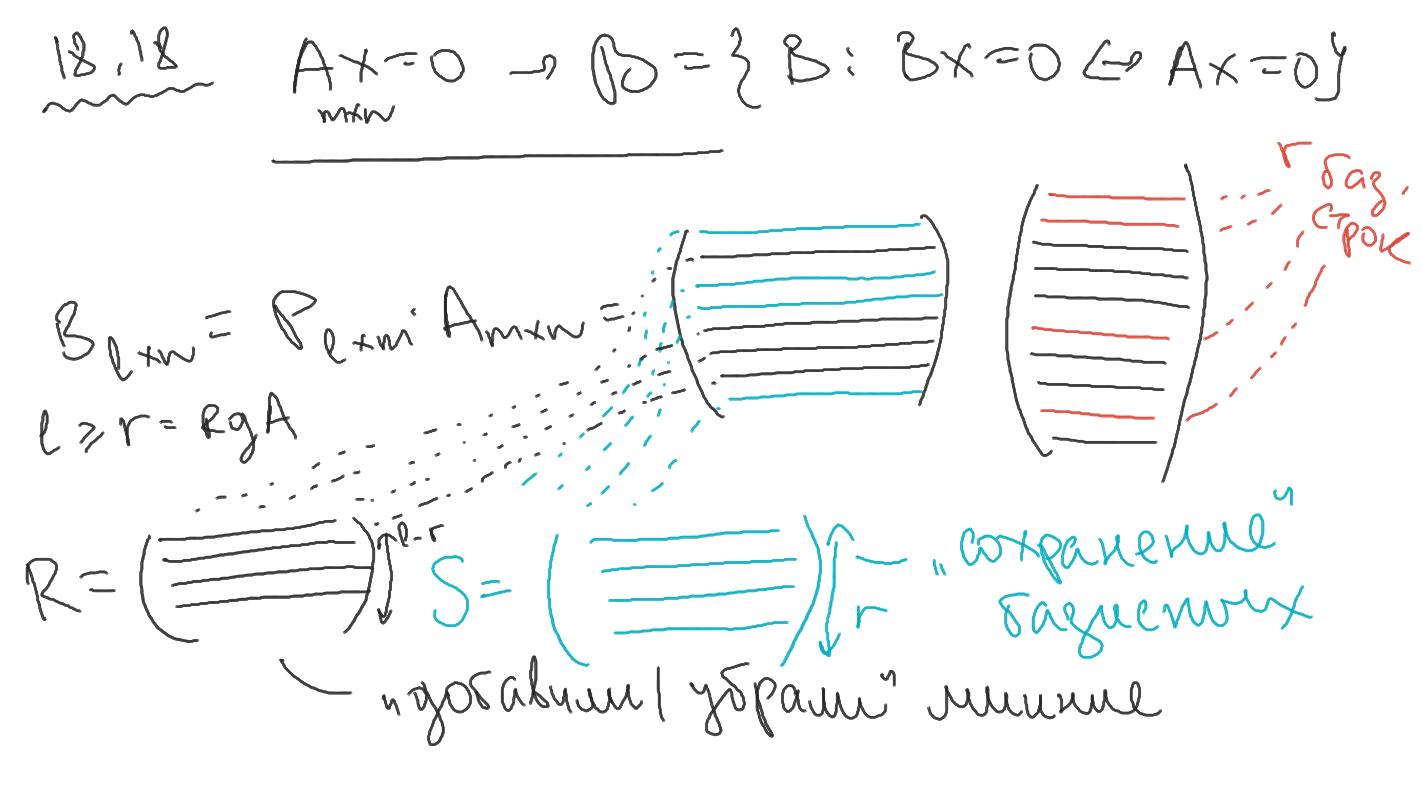
\includegraphics[width=0.8\columnwidth]{18.18.png}
    
      \caption{Подходит любая матрица $B$ вида $B \hm= PA$, где строчный ранг $P$ такой же, как у $A$ (равный $r$).
      И подматрица $S$ матрицы $P$, расположенная в $r$ базисных строках~---~это матрица, которая преобразует $r$ базисных строк матрицы $A$.}
      \label{fig:colourful-rows}
    \end{figure}
    
    \paragraph{P.S.}
    В конце задачника ответ сформулирован немного по-другому.
    Видимо, там считали, что строки матрицы $A$ линейно независимы (хотя в условии задачи про это не сказано).
    Если же строки $A$ линейно зависимы, то среди столбцов $P$ могут быть хоть нулевые (например, столбец, который во всех строках $B$ зануляет строку $A$, являющуюся линейной комбинацией базисных).
  \end{solution}
\end{document}
